% Appendix A

\renewcommand{\appendixname}{Anexo}
\chapter{Ataque con perturbaciones aleatorias FASHION MNIST. 
} % Main appendix title

\label{AppendixA} % For referencing this appendix elsewhere, use \ref{AppendixA}

Ejemplos adversarios de ataque con perturbaciones aleatorias a un modelo CNN, clasificador del conjunto de datos FASHION MNIST, con epsilon (magnitud de perturbación) 0.05, 0.1, 0.2 y 0.5. En rojo los ataques efectivos. Las imágenes generadas con epsilon 0.5 no serían consideradas como  ejemplos adversarios, ya que la perturbación es perceptible a la vista humana.
\begin{figure}[!h]
    \centering
    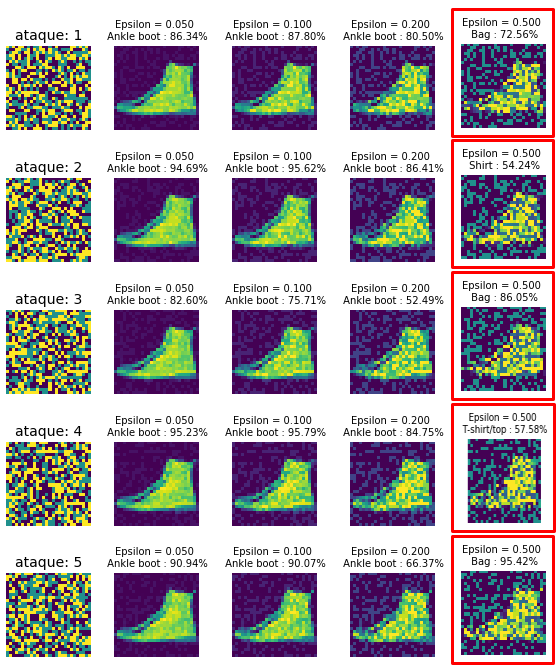
\includegraphics[scale = 0.85]{Figures/figura_67_1.PNG}
    \label{fig:67_1}
\end{figure}

\begin{figure}[!h]
    \centering
    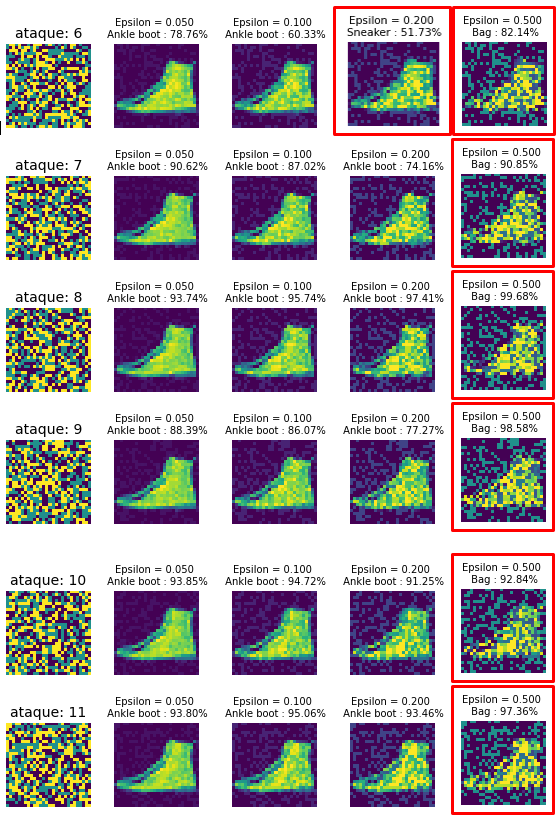
\includegraphics[scale = 0.85]{Figures/figura_67_2.PNG}
    \label{fig:67_2}
\end{figure}

\begin{figure}[!h]
    \centering
    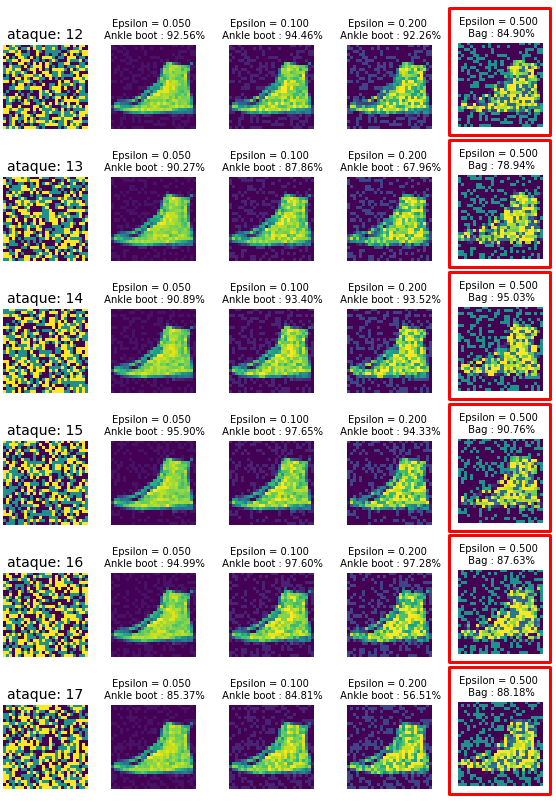
\includegraphics[scale = 0.85]{Figures/figura_67_3.PNG}
    \label{fig:67_3}
\end{figure}

\begin{figure}[!h]
    \centering
    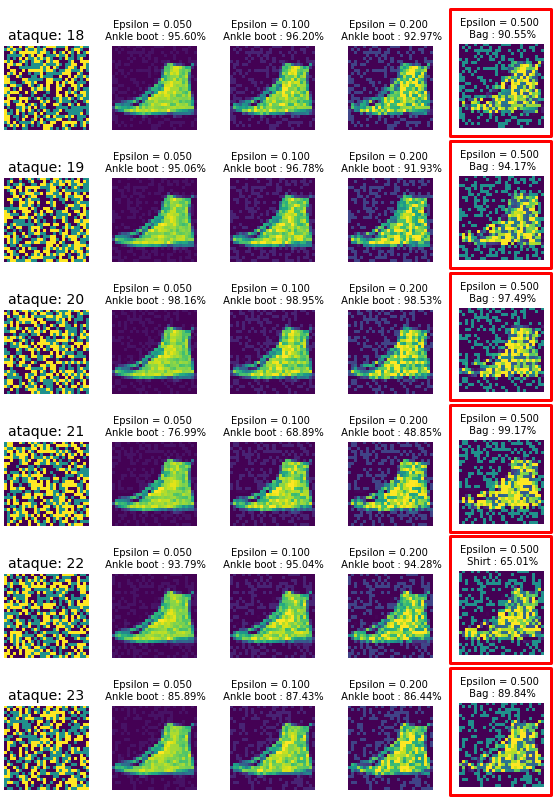
\includegraphics[scale = 0.85]{Figures/figura_67_4.PNG}
    \label{fig:67_4}
\end{figure}

\begin{figure}[!h]
    \centering
    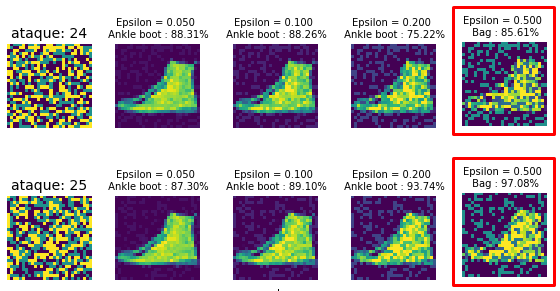
\includegraphics[scale = 0.85]{Figures/figura_67_5.PNG}
    \decoRule
    \caption[Ataque con perturbaciones aleatorias]{Ataque con perturbaciones aleatorias a modelo clasificador del conjunto de datos de FASHION MNIST.}
    \label{fig:6_5}
\end{figure}